\documentclass[a4paper,utf8]{article}
\usepackage{rapport}
\usepackage[normalem]{ulem}
\usepackage{amsfonts}
\usepackage{graphicx}
\usepackage{MnSymbol,wasysym}
\usepackage{hyperref}
\usepackage[french]{babel}


\formation{L3MI}
\date{}
\matiere{Conception Orient�e Objet}
\titre{Othello - Compte Rendu}

\newcommand\code[1]{\textsf{#1}}
\newcommand\srdjan[1]{{\color{red} #1}}

\begin{document}

\entete


\section{Ce qui a �t� impl�ment�}


-Jeu othello fonctionnel en MVC.\\%
-Nombre de cases variables.\\%
-Impl�mentation d\textquotesingle une IA (Possibilit� de choisir).\\%
-Impl�mentation d\textquotesingle un syst�me de sauvegarde utilisant des fichiers XML.\\%
-Affichage des coups disponibles pour un joueur durant son tour.\\%

\section{Structure du fichier XML}


L\textquotesingle utilisateur peut � tout moment de la partie sauvegarder l\textquotesingle �tat de celle-ci.\\%
Une g�n�ration d\textquotesingle un fichier XML aura alors lieu, et la partie sera quitt�e apr�s sa g�n�ration.\\%
\\%
Lors du chargement de la partie, on reprendra le fichier pr�c�demment cr�� et on ex�cutera le parsing en fonction de la structure afin de r�cup�rer le mod�le.\\%

Ci-dessous la structure du fichier\\%
Une grille contiendra :\\%
-Un nombre de case en abscisse\\%
-Un nombre de case en ordonn�e\\%
-Le type du joueur 1 et 2\\%
-Un ensemble de cases ayant pour identifiants une coordonn�e (x,y) et une valeur de case.\\%

\makebox[\textwidth]{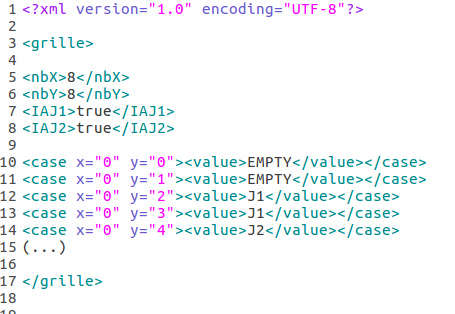
\includegraphics[width=200pt]{img/xml}}

\newpage

\section{Impl�mentation de l\textquotesingle IA}

Lors du tour de l\textquotesingle IA, celle-ci va calculer pour chaque coups possibles le nombre de cases qu\textquotesingle elle va obtenir en r�alisant celui-ci.\\%
Elle va ensuite choisir la case lui conf�rant le plus de cases.\\%


\makebox[\textwidth]{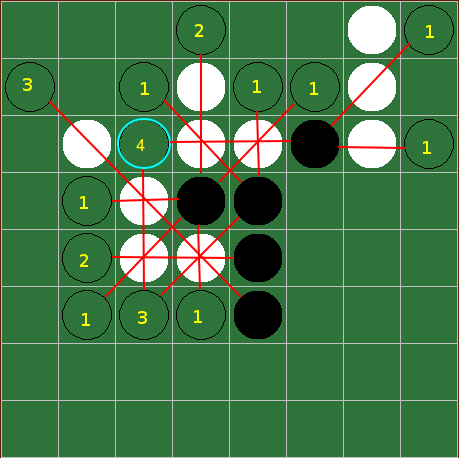
\includegraphics[width=200pt]{img/IA}}


\end{document}